\section{Ejercicio 7}
\subsection{Desarrollo}
En \'este ejercicio deb\'amos deducir que caracter\'isticas ten\'ia el $SchedMistery$ y reproducir su c\'odigo en $SchedNoMistery$. Para lo primero creamos varios lotes donde incl\'amos muchas tareas del mismo tipo, y luego hicimos combinaciones de tipos de tareas.

Al completar \'esta serie de tests pudimos deducir las caracter\'isticas que enumeramos a continuaci\'on. Llamaremos E a los valores que se le pasa al scheduler.\\


\begin{enumerate}[(a)]

\item $SchedMistery$ es un scheduler de Multiples Colas con prioridad.

\item Siendo N la cantidad de entradas que se le da al programa (\#E), el SchedMistery tendr\'a N+1 colas de prioridad, siendo la primera de 1 tick y el quantum del resto corresponde a los valores ingresados.

\item La cola de quantum 1 es la de mayor prioridad y el resto de colas va decendiendo su prioridad en el orden que se ingresan.

Ej: Siendo prioridad N+1 la m\'as alta
\begin{table}[H]
\centering
\begin{tabular}{ | c | c | c |}
  \hline			
  Cola N$^{ro}$ & quantum & prioridad\\
  \hline
1 	& 1 			& N+1\\
2 	& $E_1$ 		& N\\
3 	& $E_2$ 		& N-1\\
4 	& $E_3$ 		& N-2\\
5 	& $E_4$ 		& N-3\\
  \hline
i 	& $E_{i-1}$ 	& N-i+2\\
  \hline
N+1 & $E_N$ 		& 1\\
  \hline

\end{tabular}
\end{table}

\item Siempre se ejecuta la primer tarea en Ready de la cola no vac\'ia de mayor prioridad.

\item Si una tarea corre el quantum completo (i.e. no se bloquea o termina) y hay una cola de prioridad menor, la tarea es eliminada de la cola E$_i$ en la que se encuentra y pasa a la cola E$_{i+1}$.\\
	Si estaba en la cola de prioridad 1 (i.e. la \'ultima cola), se queda en ella.
	
\item Las tareas que corren el quantum completo en la \'ultima cola pasan al final de la cola, funcionando como un $Round Robin$ con el quantum de \'esa cola.
	
\item Si una tarea es bloqueada, es eliminada de la cola en la que se encuentra y pasa a la cola E$_{i-1}$ salvo que se encuentre en la primer cola. En cuyo caso se la vuelve a agregar al final de la misma.

\end{enumerate}

\subsubsection{Ejemplos y tests}

Los siguientes son 3 lotes de tareas que ejemplifican las propiedades antes mencionadas. Los lotes reales que se usaron para la deducci\'on son muchos y variados, y no aportan mayor informaci\'on que los presentados a continuaci\'on:\\
\newpage
Lote loteEj7a.tsk:
\begin{table}[H]
\begin{tabular}{ | l |}
  \hline
TaskCPU 30\\
TaskCPU 30\\
TaskCPU 30\\
TaskConsola 5 3 3\\
TaskConsola 5 3 3\\
  \hline
\end{tabular}
\end{table}

\begin{figure}[H]
  \centering
    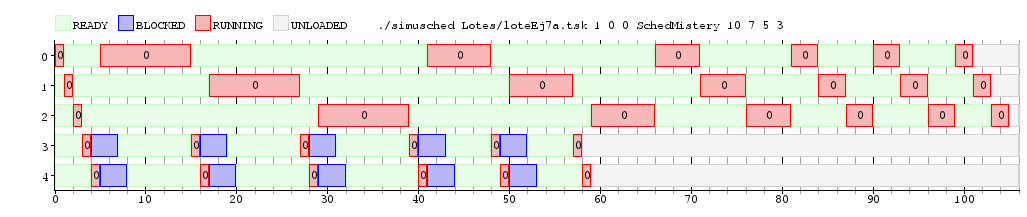
\includegraphics[width=1.1\textwidth]{imagenes/test3ej7.png}
 \caption{loteEj7a.tsk}
  \label{fig:ej7a}
\end{figure}

En \'esta figura se puede ver como el algoritmo hace ejecutar a las tareas TaskCPU primero 1 tick y luego la cantidad de ticks pasados como argumento. Finalmente, luego de hacer la primer corrida de 3 ticks vuelven a correr la misma cantidad como en un RR.

En las tareas TaskConsola s\'olo se observa que tienen mayor prioridad luego de la primer corrida, y que al estar bloqueadas dan paso a las tareas de menor prioridad.\\



Lote loteEj7b.tsk:
\begin{table}[H]
\begin{tabular}{ | l |}
  \hline
TaskCPU 50\\
TaskCPU 70\\
TaskBatch 70 3\\
@40:\\
TaskIO 40 25\\
TaskIO 15 35\\
@120:\\
TaskCPU 40\\
TaskCPU 35\\
  \hline
\end{tabular}
\end{table}

\begin{figure}[H]
  \centering
    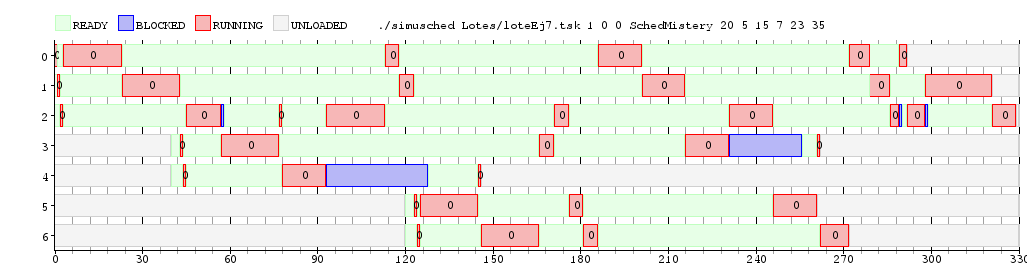
\includegraphics[width=1.1\textwidth]{imagenes/test1ej7.png}
  \caption{loteEj7b.tsk}
  \label{fig:ej7b}
\end{figure}

En la figura \ref{fig:ej7b} se puede observar adem\'as de los comportamientos antes mencionados que las tareas bloqueadas pasan a la cola siguiente 
de mayor prioridad. \'Esto se observa siguiendo las prioridades de las tareas bloqueadas, principalmente la tarea TaskBatch.\\



Lote loteEj7c.tsk:
\begin{table}[H]
\begin{tabular}{ | l |}
  \hline
TaskBatch 80 2\\
TaskBatch 80 2\\
TaskBatch 80 2\\
TaskBatch 80 2\\
  \hline
\end{tabular}
\end{table}

\begin{figure}[H]
  \centering
    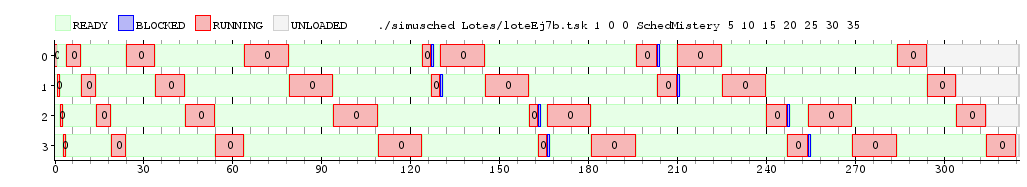
\includegraphics[width=1.1\textwidth]{imagenes/test2ej7.png}
  \caption{loteEj7c.tsk}
  \label{fig:ej7c}
\end{figure}


Para ejemplificar mejor lo antes dicho creamos este caso donde s\'olo se ejecutan TaskBatch. Con esto podemos ver los cambios de prioridad de las tareas.


\subsection{Experimentación}

Veremos que el $SchedNoMistery$ se comporta igual que el $SchedMistery$:

La ejecuci\'on de $SchedNoMistery$ para los ejemplos anteriores son efectivamente los mismos:

\begin{figure}[H]
  \centering
    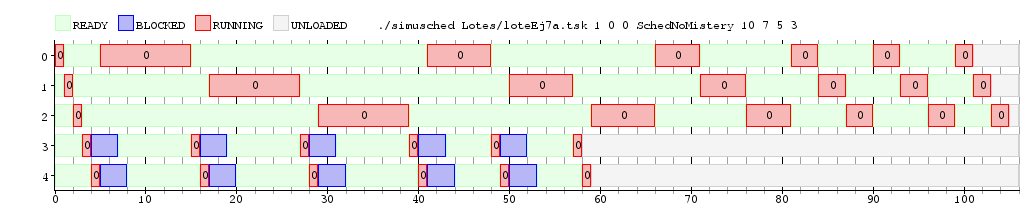
\includegraphics[width=1.1\textwidth]{imagenes/Ej7verif1.png}
 \caption{loteEj7a.tsk con SchedNoMistery}
  \label{fig:ej7aNo}
\end{figure}

\begin{figure}[H]
  \centering
    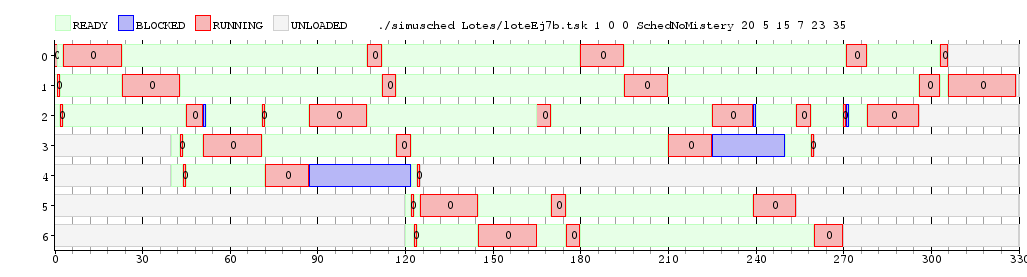
\includegraphics[width=1.1\textwidth]{imagenes/Ej7verif2.png}
 \caption{loteEj7b.tsk con SchedNoMistery}
  \label{fig:ej7bNo}
\end{figure}

\begin{figure}[H]
  \centering
    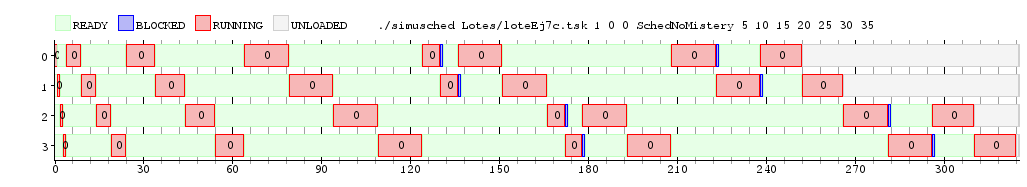
\includegraphics[width=1.1\textwidth]{imagenes/Ej7verif3.png}
 \caption{loteEj7c.tsk con SchedNoMistery}
  \label{fig:ej7cNo}
\end{figure}

Se puede observar que s\'olo se comportan distintos los TaskBatch. Pero eso es porque TaskBatch se bloquea de forma pseudo-aleatoria, seg\'un sus par\'ametros.
